\documentclass[a4paper,titlepage]{article}
\usepackage[utf8]{inputenc}
\usepackage{fullpage}
\usepackage{indentfirst}
\usepackage[per-mode=symbol]{siunitx}
\usepackage{listings}
\usepackage{graphicx}
\usepackage{color}
\usepackage{amsmath}
\usepackage{array}
\usepackage[hidelinks]{hyperref}
\usepackage[format=plain,font=it]{caption}
\usepackage{subcaption}
\usepackage{standalone}
\usepackage[nottoc]{tocbibind}
\usepackage[noabbrev,capitalize,nameinlink]{cleveref}
\usepackage{listings}
\usepackage{xspace}
\usepackage{tikz}
\usepackage{circuitikz}
\usepackage{titlesec}
\usepackage[cache=false]{minted}
\usepackage{booktabs}
\usepackage{csvsimple}
\newcommand{\MATLAB}{\textsc{Matlab}\xspace}
\usepackage{siunitx}
\usepackage[super]{nth}
\usepackage[titletoc]{appendix}

% Custom commands
\newcommand\numberthis{\addtocounter{equation}{1}\tag{\theequation}}
\newcommand{\code}[1]{\texttt{#1}}
\newcolumntype{P}[1]{>{\centering\arraybackslash}p{#1}}

\setminted{linenos,breaklines,fontsize=auto}

%\titleformat*{\section}{\normalsize\bfseries}
%\titleformat*{\subsection}{\small\bfseries}
\renewcommand{\thesubsection}{\thesection.\alph{subsection}}
\providecommand*{\listingautorefname}{Listing}
\newcommand*{\Appendixautorefname}{Appendix}


\begin{document}
	\sloppy	
	
	\begin{center}
		{\LARGE \bf ECSE 597: Circuit Simulations and Modeling}\\
		{\large Assignment 2, \quad \today}\\
		{\large Wenjie Wei, 260685967}
	\end{center}

	\section{Circuit Diagram}
		Figure \ref{circuit} below shows the circuit described in the file \texttt{\textbf{Circuit\_diodeckt1.m}}.
		
		\begin{figure}[!h]
			\centering
			\begin{circuitikz}[american voltages]
				\draw
				(0, 3)node[label={[font=\footnotesize]above:$N_1$}]{} to [V, l=$2V$,*-*] (0, 0) 
				(0, 3) to [R, l=$50\Omega$, *-*] (3, 3) node[label={[font=\footnotesize]above:$N_2$}]{}
				to [R, l=$50\Omega$, *-*] (3,0)
				(3, 3) to [short, *-*] (6, 3)
				to [C, l=$1\mu F$, *-*] (6, 0)
				(0, 3) to [short, *-*] (0, 4.5)
				to [Do, l=$I_s(e^{(v/v_t)} - 1)$, *-*] (3, 4.5)
				to [short, *-*] (3, 3)
				(0, 0) to [short,  *-*] (3, 0) node[ground]{}
				to [short, *-*] (6, 0)
				;
			\end{circuitikz}
			\caption{Circuit described in \normalfont \texttt{\textbf{Circuit\_diodeckt1.m}}}
			\label{circuit}
		\end{figure}
	
		Where $I_s = 1\times10^{-15}A$, $V_t = 26\times10^{-3}V$.
		
	\section{Simulation Results}
		The result computed after running the test bench is:
		$$
			V_1 = 2V,\quad V_2 = 1.2245V
		$$
		and the current flowing through the voltage source is calculated to be:
		$$
			I_E = -0.0245A
		$$
		defining that the direction of the current is from Node 1 to ground. 
	\section{Plotting Result}
		Figure \ref{result} below shows the plotting result of the norm of $\Delta x$ after each iteration. 
		\begin{figure}[H]
			\centering
			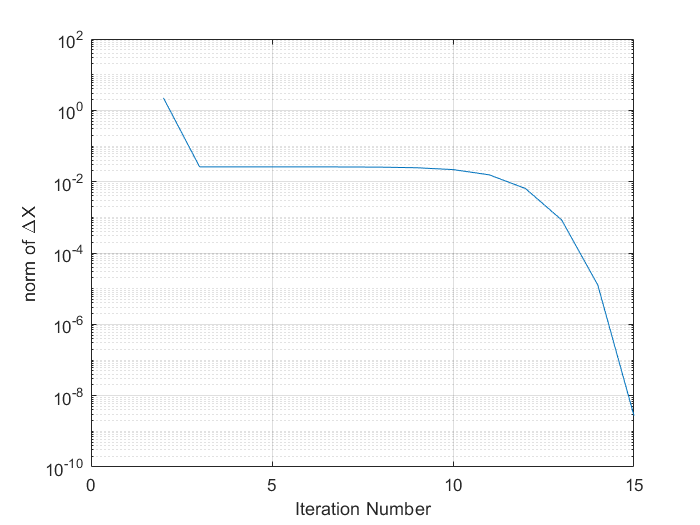
\includegraphics[width=0.5\linewidth]{result}
			\caption{Plotting Results of the Norm of $\Delta x$ After Newton-Raphson Iterations}
			\label{result}
		\end{figure}
	\begin{appendices}
		
		\section{Code Listings} \label{appendix:code}
		
		\setminted{linenos,breaklines,fontsize=\footnotesize}
		
		\begin{center}
			\captionof{listing}{MATLAB Function Calculating the Jacobian (\texttt{nlJacobian.py}).}
			\inputminted{matlab}{../../src/a2/nlJacobian.m}
			\label{jacobian}
		\end{center}
		
		\begin{center}
			\captionof{listing}{MATLAB Function Performing DC Simulation (\texttt{dcsolve.py}).}
			\inputminted{matlab}{../../src/a2/dcsolve.m}
			\label{dc}
		\end{center}
	\end{appendices}
\end{document}